\subsection{Entity-Relationship Schema}


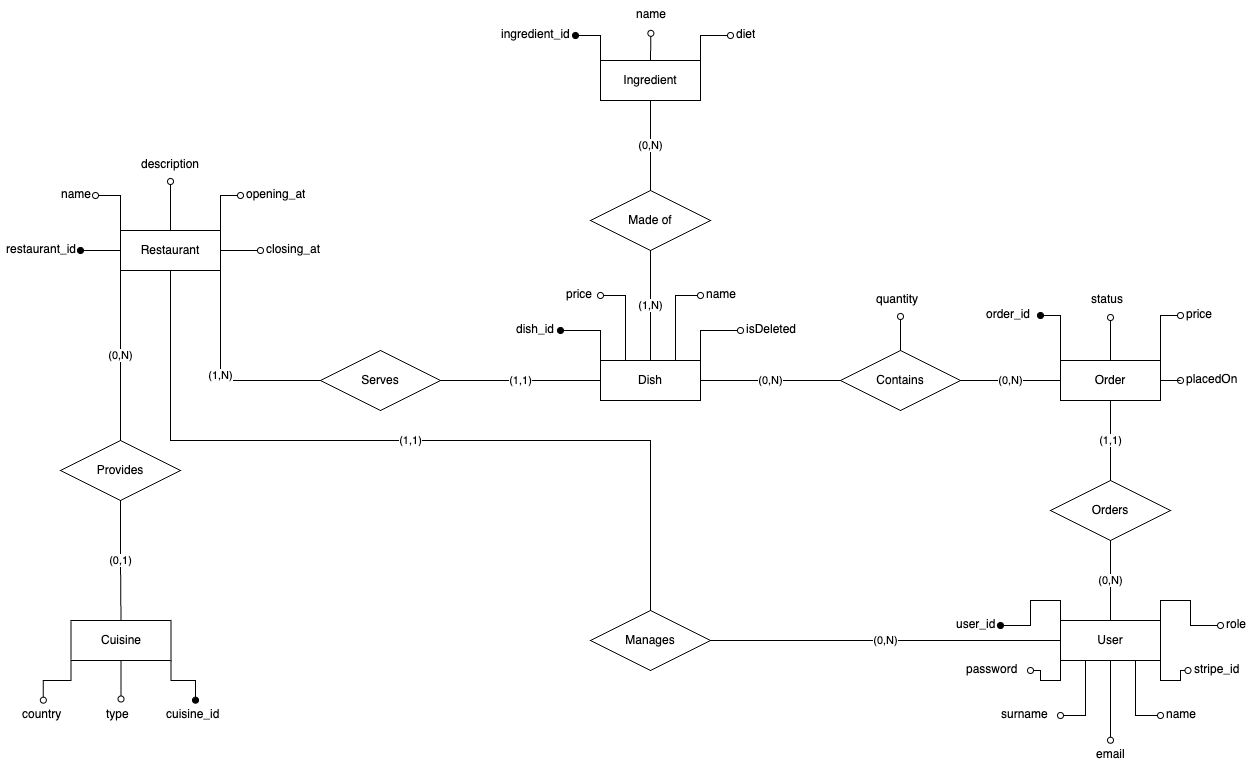
\includegraphics[width=1.0\textwidth]{resources/ER-diagram.png}


%Describe here your ER schema


We have 6 entities in the schema:
\begin{itemize}
    \item \textbf{Restaurant}: each restaurant is defined by \textit{restaurant\_id} which is of type SERIAL. Then we have \textit{name} and \textit{description} of type VARCHAR, in conclusion we have \textit{opening\_at} and \textit{closing\_at} which are of type TIME and describe the opening and the closing hour respectively.
    
    \item \textbf{Cuisine}: it expresses the type of cuisine that a restaurant provides. It is defined by \textit{cuisine\_id} which is of type SERIAL. Then \textit{type} which is of type VARCHAR and expresses the type of food the cuisine provides. In conclusion, \textit{country} whose value is selected between a finite set of 239 countries inside an ENUM type.

    \item \textbf{Dish}: each dish is defined by \textit{dish\_id} which is of type SERIAL. Then we have \textit{price} which is of type REAL, \textit{name} which is of type VARCHAR and \textit{isDeleted} which is of type BIT and represents if a dish has been deleted or not, the dish cannot be literally deleted by the database otherwise orders' history consistency would not hold.

    \item \textbf{Ingredient}: each ingredient is defined by \textit{ingredient\_id} which is of type SERIAL. Then \textit{name} is of type VARCHAR, \textit{diet} whose value is selected between a finite set of 3 values ("vegan", "vegetarian", "carnivorous") inside an ENUM type.

    \item \textbf{Order}: each order is defined by \textit{order\_id} of type SERIAL. Then \textit{price} of type REAL which is the weighted sum of the prices of the dishes in the order, where the weights are the quantities of each dish, \textit{placedOn}, of type TIMESTAMP, defines the day and time at which an order has been placed, then \textit{status} whose value is selected between a finite set of 2 elements ("pending", "completed") inside an ENUM type.

    \item \textbf{User}: each user is defined by \textit{user\_id} which is of type SERIAL. Then \textit{email} is of type VARCHAR and it's value is unique within the table, \textit{name} and \textit{surname} which are of type VARCHAR, \textit{stripe\_id} which is of type VARCHAR and it is necessary to perform a payment, \textit{role} which is of type VARCHAR and takes value between a finite set of 3 elements ("customer", "manager", "admin") inside an ENUM type.
    
\end{itemize}
